\section{Results}
\label{sec:results}

\subsection{Pillar C: four-anchor Hubble fit}
\label{sec:pillarC}

The core numerical result is the weighted fit of \cref{eq:hubble} to the four inputs in \cref{tab:anchors}.
The submitted manuscript quotes
\begin{equation}
  H_\infty = 104.5\,\mathrm{km\,s^{-1}\,Mpc^{-1}}\,,
  \quad
  \beta = -6.24\,\mathrm{km\,s^{-1}\,Mpc^{-1}}\,,
\end{equation}
together with $R^2 = 0.91$ and $\chi^2/\mathrm{dof} = 0.28$ (\cref{fig:jwst_h0}).
One figure caption in the submitted text prints $R^2 = 0.907$.
The notebook output prints $H_\infty = 104.469\ldots$, which rounds to the quoted $104.5$.
These are the submitted numbers.
They were not recomputed here.
With $N=4$ and two parameters the fit has $\mathrm{dof}=2$.
An unweighted $R^2$ of $0.91$ on four points, and a reduced $\chi^2$ of $0.28$ on two degrees of freedom, describe a flexible curve passing close to four assigned anchors whose error bars are not small compared with the residuals.
They do not by themselves establish a time-dependent expansion history.
The parameter covariance and the leave-one-anchor-out shifts are not reported.
\revtodo{Insert the covariance and the leave-one-anchor-out table after the refit specified in \cref{sec:fit-method}.}

\begin{figure}[htbp]
  \centering
  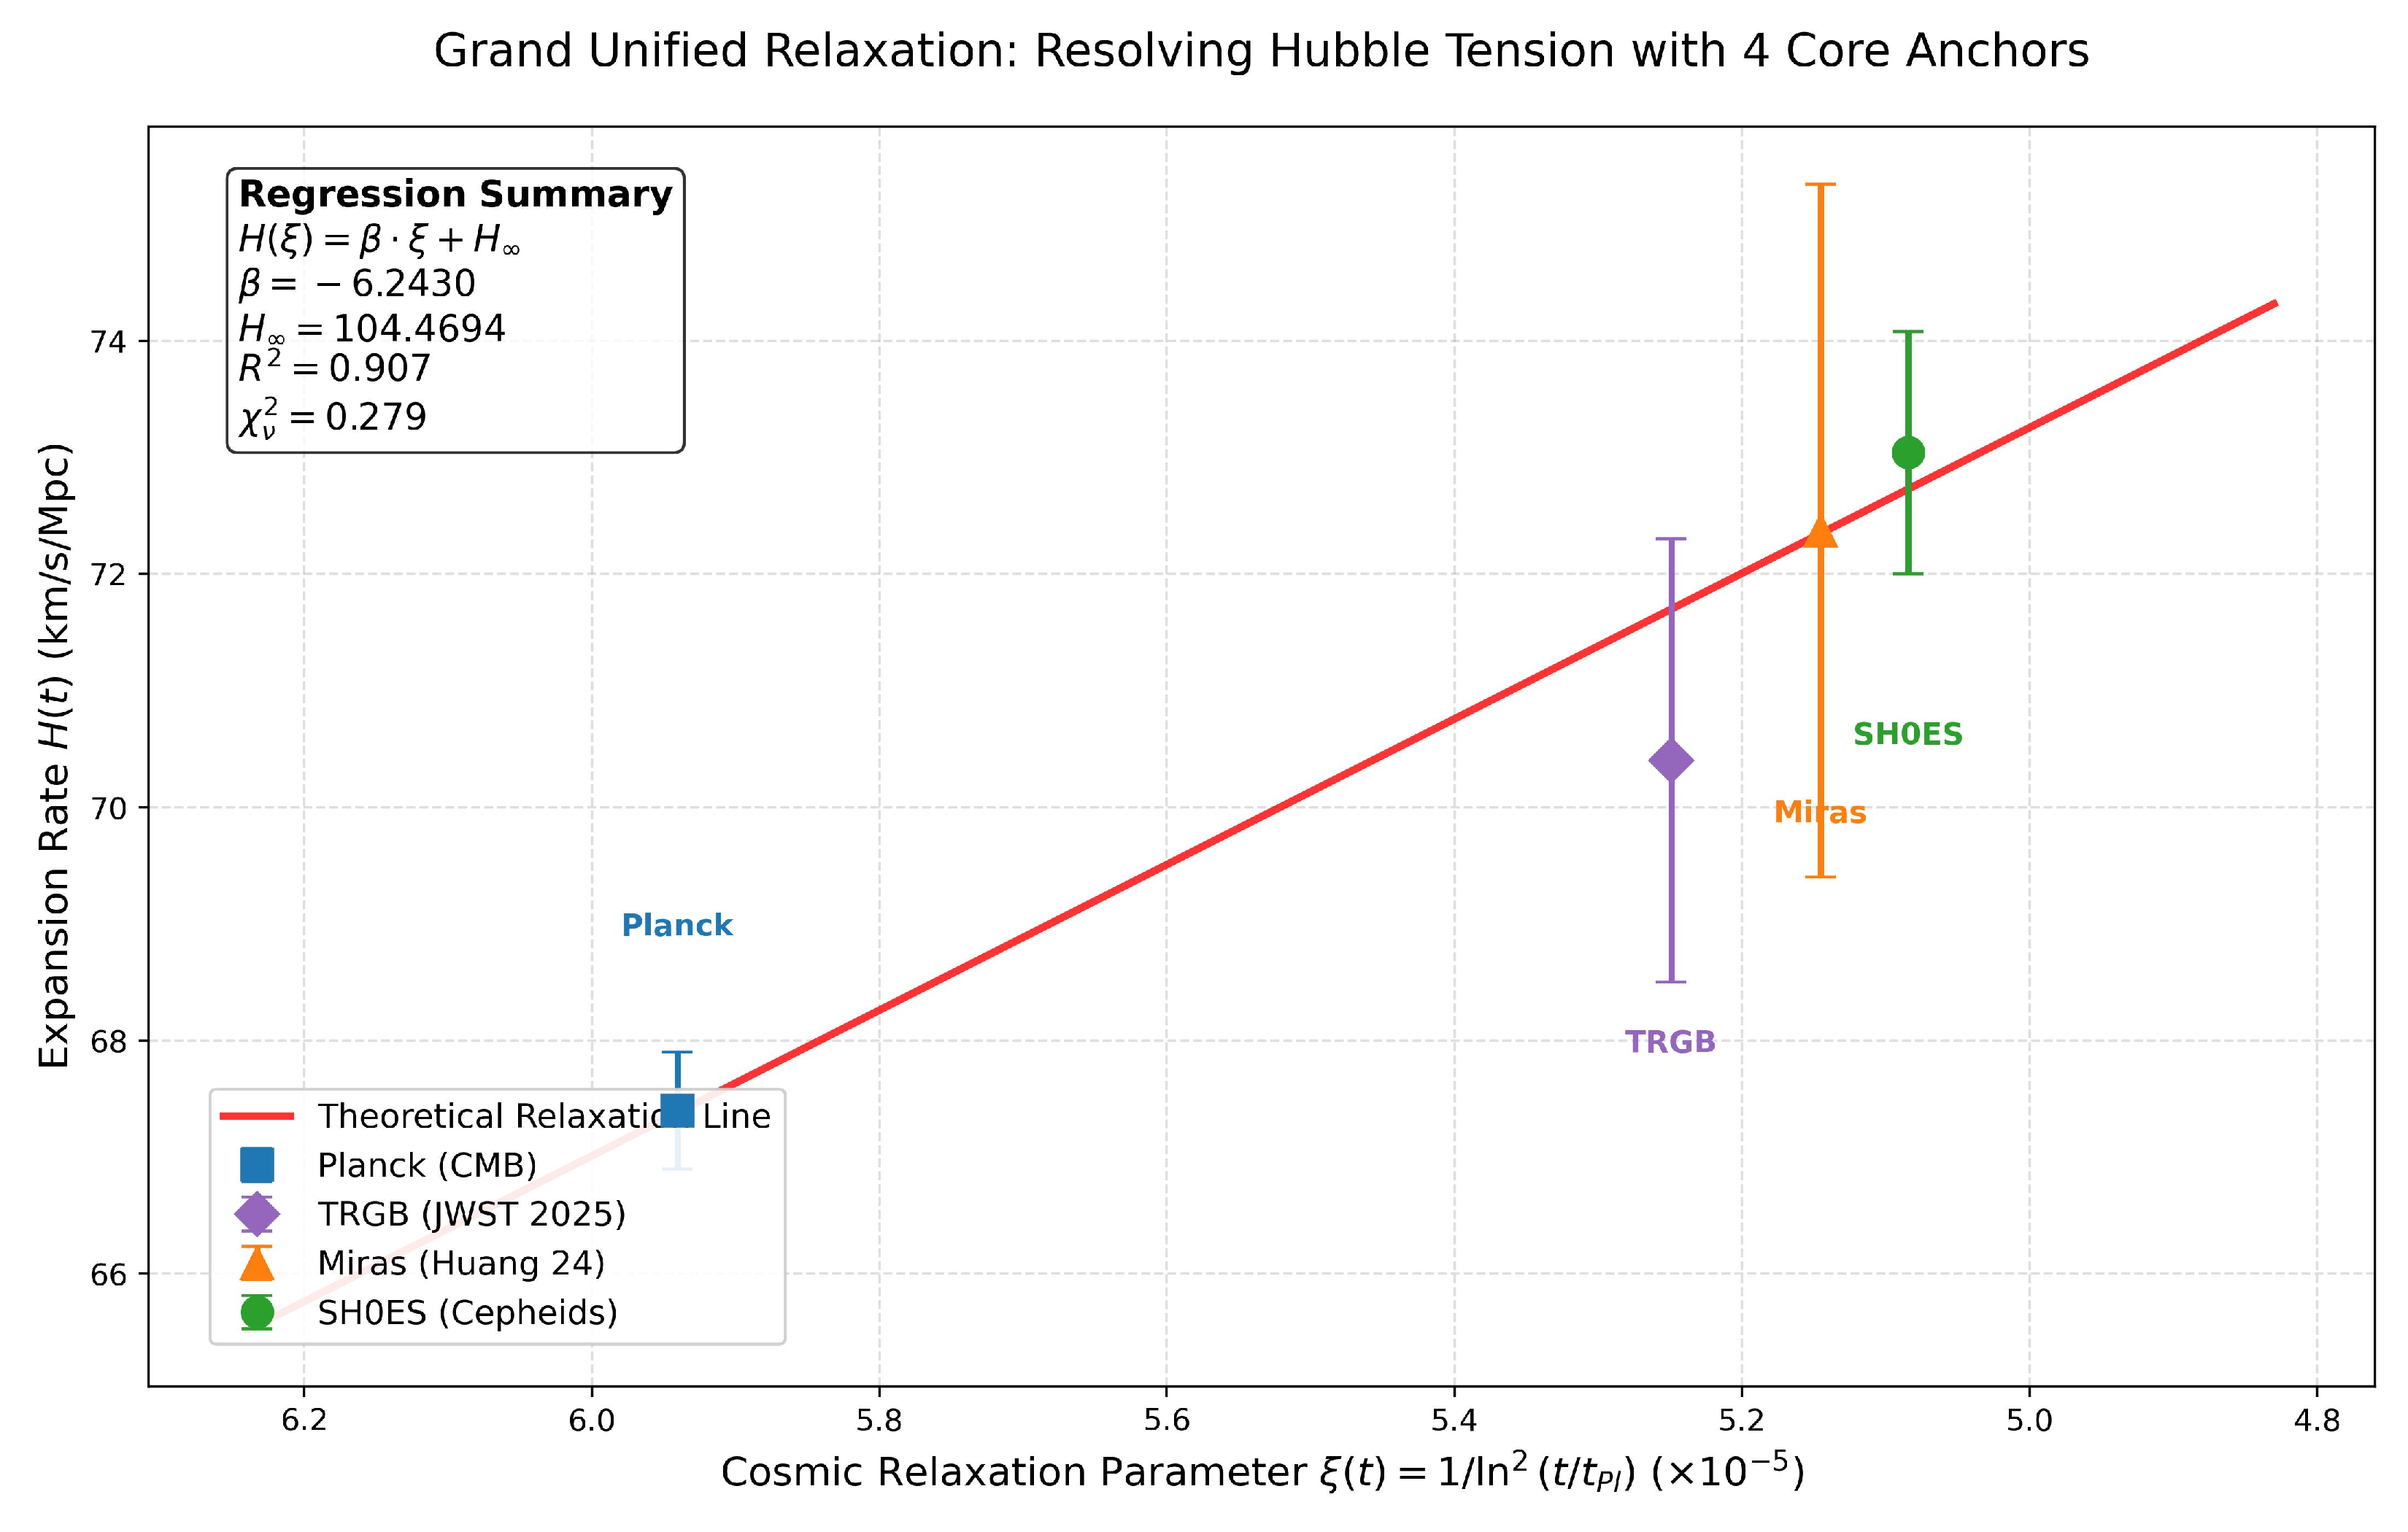
\includegraphics[width=\columnwidth]{fig19_jwst_h0_anchors.pdf}
  \caption{Curve \cref{eq:hubble} drawn through the four inputs of \texttt{fig19\_jwst\_h0\_anchors.ipynb} (\cref{tab:anchors}).
  The submitted summary of this figure is $R^2 = 0.91$ and $\chi^2/\mathrm{dof} = 0.28$ on $\mathrm{dof}=2$.
  The horizontal axis is the scaled regressor $10^{5}/\ln^2(t/\tP)$.
  The submitted prose described the anchors as SH0ES, JWST, Planck, and BAO; the notebook inputs are the four rows of \cref{tab:anchors}.
  The Planck point is a present-day $\Lambda$CDM inference placed at an assigned early time.}
  \label{fig:jwst_h0}
\end{figure}

The intercept $H_\infty$ lies above every anchor in \cref{tab:anchors}.
Inside \cref{eq:hubble} that is expected when $\beta<0$: the correction $\beta\,10^{5}\xi(t)$ is negative at finite $t$ and shrinks as $t$ increases, so the curve rises toward $H_\infty$.
The submitted high-redshift evaluations $H(z=2) = 72.1$, $H(z=5) = 71.6$, and $H(z=10) = 71.2$, in $\mathrm{km\,s^{-1}\,Mpc^{-1}}$, sit near the anchor values rather than near $104.5$ because they are finite-$t$ evaluations, as the arithmetic in \cref{sec:hubble-ansatz} shows for $z\approx 2$.
\revtodo{Recompute $H(z)$ from one shared $t(z)$, one value of $\tP$, and the confirmed $(H_\infty,\beta)$, and replace the quoted $71$--$72$ sequence only if that recomputation changes it.}

\subsection{Exploratory quasar comparison}
\label{sec:alpha}

The submitted manuscript reported fits of \cref{eq:alpha} to quasar $\Delta\alpha/\alpha$ samples.
Those fits are kept here as an exploratory side-by-side comparison and are not a detection.
\Cref{tab:alpha} copies the instrument table printed in the submitted manuscript.
\Cref{fig:alpha_quasar,fig:pillar_K_murphy} show the corresponding submitted figures.

Two incompatible Murphy-sample values appear in the submitted text.
The Pillar~A narrative quotes $\Gamma = +6.42\pm 1.14$ ($\Delta\chi^2 = 31.54$) under budget~(i).
The instrument table, the submitted abstract, and one conclusion sentence quote $\Gamma = +5.56\pm 0.99$ for the same Murphy sample under budget~(i).
The conclusion sentence also quotes $\Delta\chi^2 = 31.83$, which matches neither $31.54$ nor a unique reading of $5.56/0.99$.
This revision does not choose among these quotations.
\revtodo{Replace \cref{tab:alpha} with one refit. Until then the table is a record of the submitted quotations, and no row is a measured drift.}

On the numbers as quoted, the Keck-only rows are positive and the VLT-only rows are negative, while the full Keck+VLT union is closer to zero than the Keck-only union.
The full King et al.~(2012) catalog, treated separately in the submitted text, was quoted with reduced $\chi^2 = 0.881$ for the ansatz and $0.878$ for a constant, $\Delta\chi^2\approx 0$, and $\Delta\mathrm{BIC} = +5.7$ in favor of the constant.
No pre-registered rule selects the Keck-only subset.
The sign difference is therefore an unresolved subset dependence.
It is consistent with a Keck wavelength-calibration systematic~\citep{Whitmore2015,Wilczynska2020}, and it is also consistent with a fluctuation of that subset.
The comparison does not establish a cosmological drift of $\alpha$.

\begin{table*}[htbp]
\centering
\caption{Side-by-side quasar coefficients as quoted in the submitted manuscript, not as a new fit.
$\Gamma$ is in units of $10^{-5}$.
Budget~(i) uses the per-absorber fit error only.
Budget~(ii) adds the published random term in quadrature.
The Murphy budget~(i) row disagrees with the narrative value $+6.42\pm 1.14$ quoted in the same submitted section.
The full King et al.~(2012) catalog ($N=295$) was quoted separately as consistent with $\Gamma=0$ at $\Delta\mathrm{BIC}=+5.7$ in favor of a constant.}
\label{tab:alpha}
\small
\begin{tabular}{lcccc}
\hline
Subset & $N$ & Budget & Quoted $\Gamma\pm\sigma_\Gamma$ & Quoted ratio \\
\hline
Murphy 2003 (Keck) & 128 & (i)  & $+5.56\pm 0.99$ & $+5.64$ \\
                   & 128 & (ii) & $+5.08\pm 1.81$ & $+2.81$ \\
King 2012 Keck-only & 141 & (i)  & $+6.28\pm 0.97$ & $+6.47$ \\
                    & 141 & (ii) & $+6.40\pm 1.94$ & $+3.31$ \\
King 2012 VLT-only  & 154 & (i)  & $-2.35\pm 0.63$ & $-3.72$ \\
                    & 154 & (ii) & $-2.05\pm 1.14$ & $-1.79$ \\
Keck union          & 269 & (i)  & $+5.92\pm 0.69$ & $+8.57$ \\
                    & 269 & (ii) & $+5.70\pm 1.32$ & $+4.31$ \\
Keck+VLT union      & 423 & (i)  & $+1.42\pm 0.47$ & $+3.04$ \\
                    & 423 & (ii) & $+1.27\pm 0.86$ & $+1.47$ \\
\hline
\end{tabular}
\end{table*}

\begin{figure}[htbp]
  \centering
  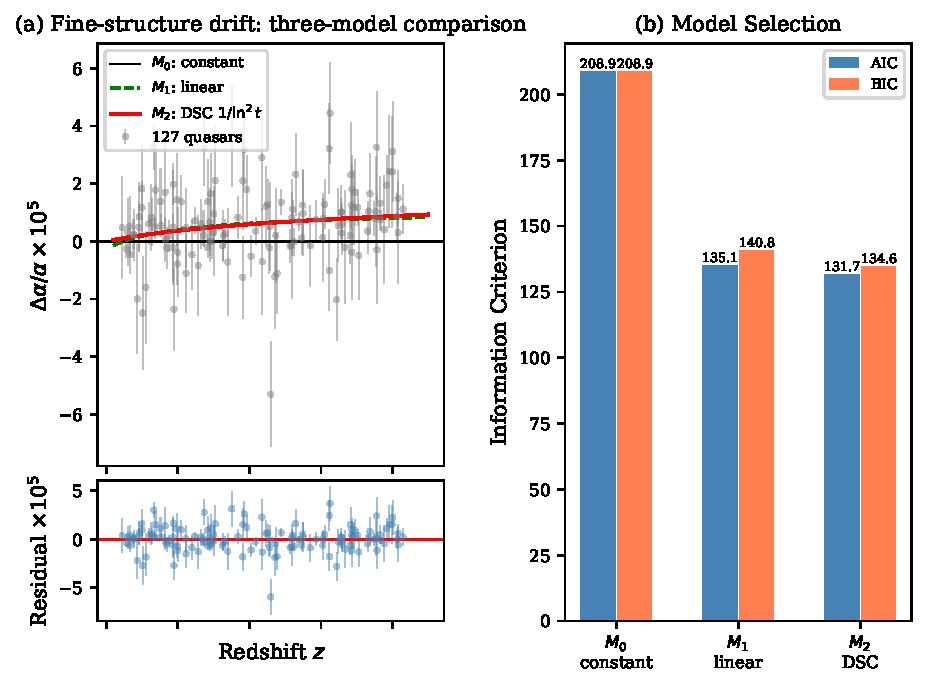
\includegraphics[width=\columnwidth]{fig18_alpha_drift_quasar.pdf}
  \caption{Exploratory $\Delta\alpha/\alpha$ comparison on the Murphy et al.~(2003) Keck/HIRES sample, as plotted for the submitted manuscript.
  The submitted caption attached a $5.6\sigma$ claim to this figure.
  That claim is withdrawn.
  The Murphy coefficient in this figure was not reconciled with \cref{tab:alpha}.}
  \label{fig:alpha_quasar}
\end{figure}

\begin{figure}[htbp]
  \centering
  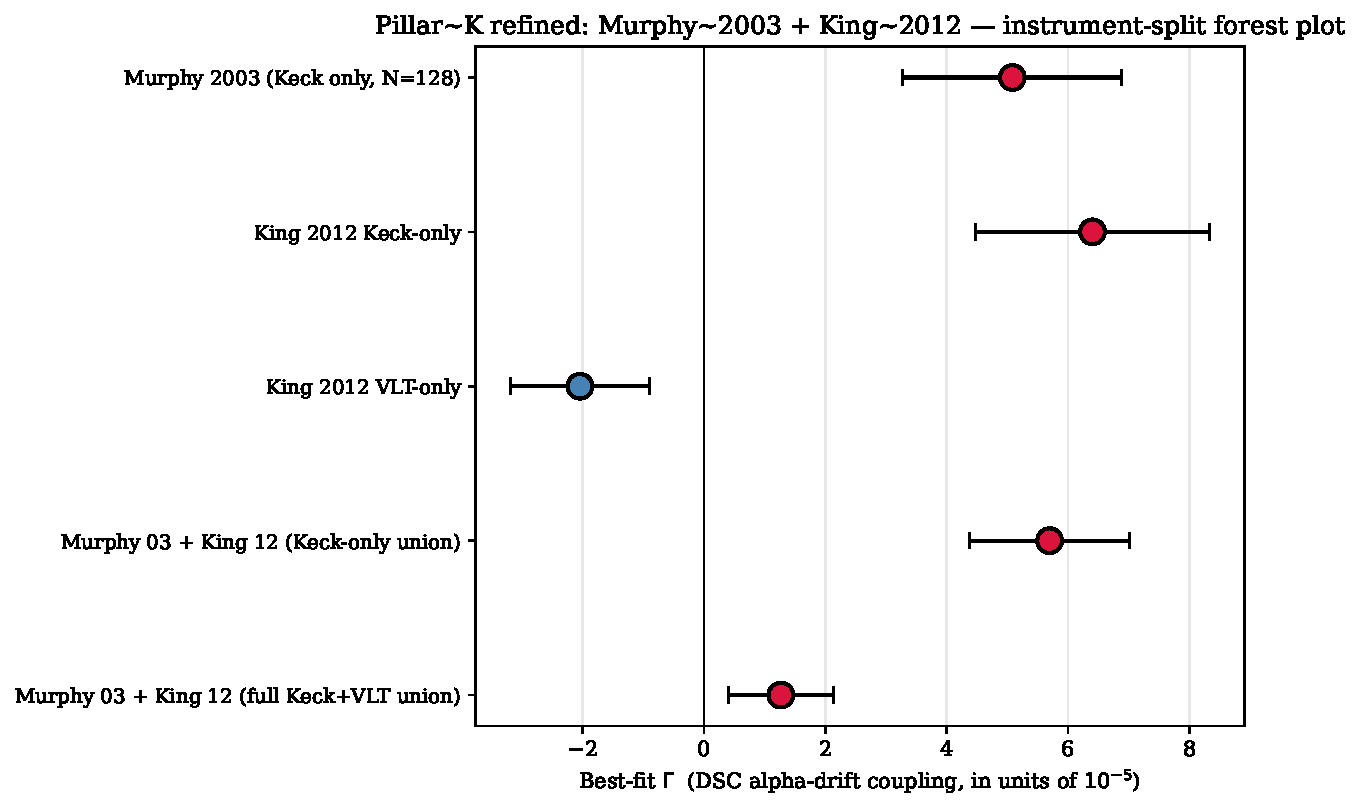
\includegraphics[width=\columnwidth]{fig28_pillar_K_murphy_forest.pdf}
  \caption{Exploratory forest plot of the quoted $\Gamma$ values across the Keck-only, VLT-only, and combined subsets.
  Positive Keck-only values and a negative VLT-only value are both present in the submitted table.
  The plot is a subset comparison, and it is not a detection of a cosmological drift.}
  \label{fig:pillar_K_murphy}
\end{figure}

\subsection{Dense late-time samples}
\label{sec:dense}

\Cref{tab:dense} collects $\chi^2/\mathrm{dof}$ values quoted in the submitted manuscript for late-time samples.
They were not recomputed.
Where the ansatz returns a larger $\chi^2$ than flat $\Lambda$CDM, the ansatz is a worse description of that sample.
The DESI DR2 entry, $\chi^2/\mathrm{dof}\sim 10^3$, is a poor goodness of fit.
This revision does not read it as evidence that the ansatz is correct, and it does not read it as a confirmation of low-redshift degeneracy.
The same statement applies to the cosmic-chronometer, Pantheon$+$, and joint entries.
A Fisher forecast quoted in the submitted text, based on compressed Planck observables and DESI BAO ratios, gave $\sigma(\gamma_{\mathrm{eff}})\sim 10^{4}$ and therefore did not measure $\gamma$.
Five elementary background checks (positive $H^2$, $\dot H<0$, monotone growth of a density contrast, a prescribed $c_s^2=0$, and $w_{\mathrm{eff}}(z=0)$ near the $\Lambda$CDM value) were reported as passed for a limited parameter window.
Those checks do not address perturbative stability or gradient instabilities.
\revtodo{Recompute \cref{tab:dense} under the common likelihood requested in \cref{sec:late-method}. Perturbative and gradient stability calculations are not in this revision.}

\begin{table}[htbp]
\centering
\caption{Late-time goodness of fit as quoted in the submitted manuscript.
The ansatz column is a worse description wherever it exceeds the $\Lambda$CDM column.
The DESI DR2 value of order $10^3$ is a poor fit of that sample.}
\label{tab:dense}
\small
\begin{tabular}{llcc}
\hline
Label & Sample & $\Lambda$CDM & Ansatz \\
\hline
F & cosmic chronometers (32) & $0.49$ & $4.01$ \\
G & Pantheon$+$ (1580) & $0.88$ & $1.27$ \\
H & DESI DR2 BAO & $1.07$ & $\sim 10^{3}$ \\
J & joint (1623 constraints) & $0.96$ & $23.7$ \\
\hline
\end{tabular}
\end{table}

\subsection{Pillar M: dynamic range, and a falsification standard}
\label{sec:pillarM}

The submitted leverage note evaluates $10^{5}\xi(t)$ along a $\Lambda$CDM time-redshift relation and quotes $5.92$ at $z=1100$, $5.19$ at $z=1.97$, $5.09$ at $z=0.07$, and $5.08$ at $z=0$ (\cref{fig:pillar_M}).
The difference between recombination and the present is $0.84$ in these units, and the difference between $z=2$ and $z=0.07$ is $0.10$.
Their ratio, $8.4$, is a property of $\xi(t)$ under that clock.
It says that the fitting function moves more between recombination and today than it does inside $z<2$.
It does not convert a poor $\chi^2$ into supporting evidence.

The falsification standard used in this revision is the following.
The four-anchor description fails if a leave-one-anchor-out refit, once computed, misses the omitted anchor by more than the quoted uncertainty of that anchor, or if a direct $H(z)$ measurement with a stated covariance falls outside \cref{eq:hubble} by more than that measurement allows.
Separately, the ansatz fails as a description of any sample in \cref{tab:dense} for which its $\chi^2$ is unacceptable on that sample's covariance.
A non-detection in a redshift window where $\xi(t)$ is almost constant is then an unsurprising non-detection.
It is not a second success.
A detection in that window would challenge the expectation that the function is unresolved there, and it would be reported as a failure of that expectation.
Either outcome is informative.
The standard is not satisfied by accommodating both.

\begin{figure*}[htbp]
  \centering
  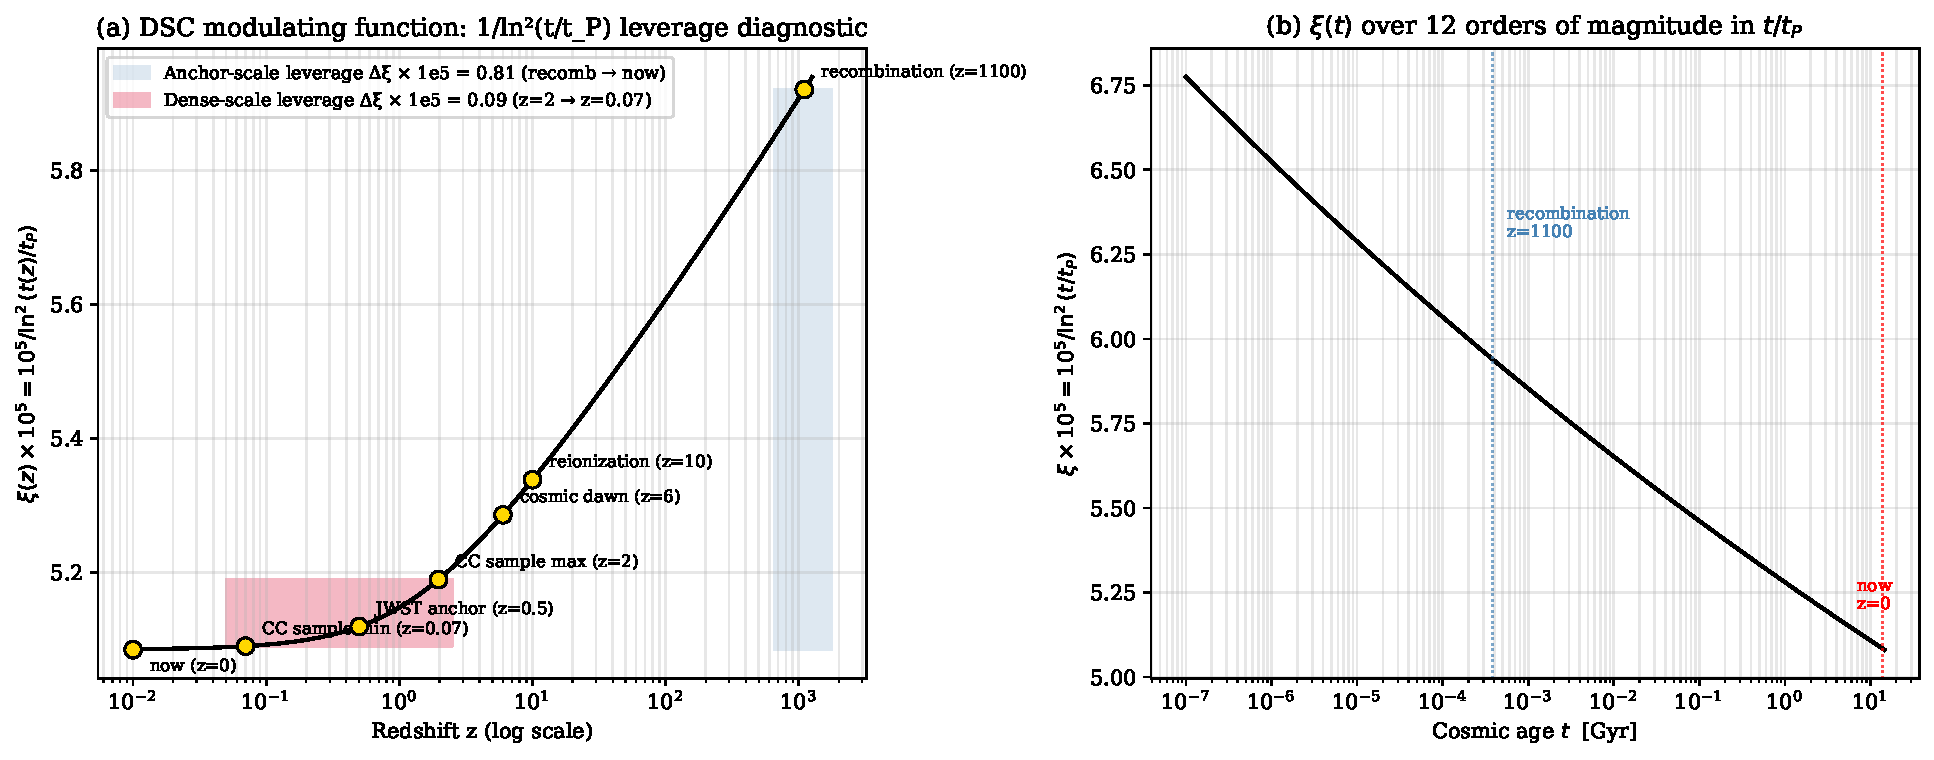
\includegraphics[width=\textwidth]{fig29_pillar_M_leverage.pdf}
  \caption{Dynamic range of $10^{5}/\ln^2(t/\tP)$ as plotted in the submitted manuscript.
  The curve records how little $\xi(t)$ changes for $z<2$ under the adopted clock.
  The figure is not a goodness-of-fit test, and the $\chi^2/\mathrm{dof}\sim 10^3$ DESI DR2 entry in \cref{tab:dense} remains a poor fit.}
  \label{fig:pillar_M}
\end{figure*}

\subsection{Pillar N: laboratory translation}
\label{sec:pillarN}

\Cref{eq:alphadot} maps a coefficient $\Gamma$ to a present-day $\dot\alpha/\alpha$.
The submitted evaluation is $|\dot\alpha/\alpha| \approx |\Gamma|\times 5.25\times 10^{-22}\,\mathrm{yr}^{-1}$, and the Rosenband et al.\ bound then reads $|\Gamma|\lesssim 1.9\times 10^{4}$ inside the ansatz~\citep{Rosenband2008}.
\Cref{fig:pillar_N} places the quoted quasar coefficients next to that conditional bound.
Because those coefficients are not reconciled (\cref{sec:alpha}), the figure is an illustration of the translation and not a combined measurement.
The laboratory bound and the quasar catalogs are not combined into a joint posterior in this revision.
The translation also does not constrain $\beta$ in \cref{eq:hubble}.

\begin{figure}[htbp]
  \centering
  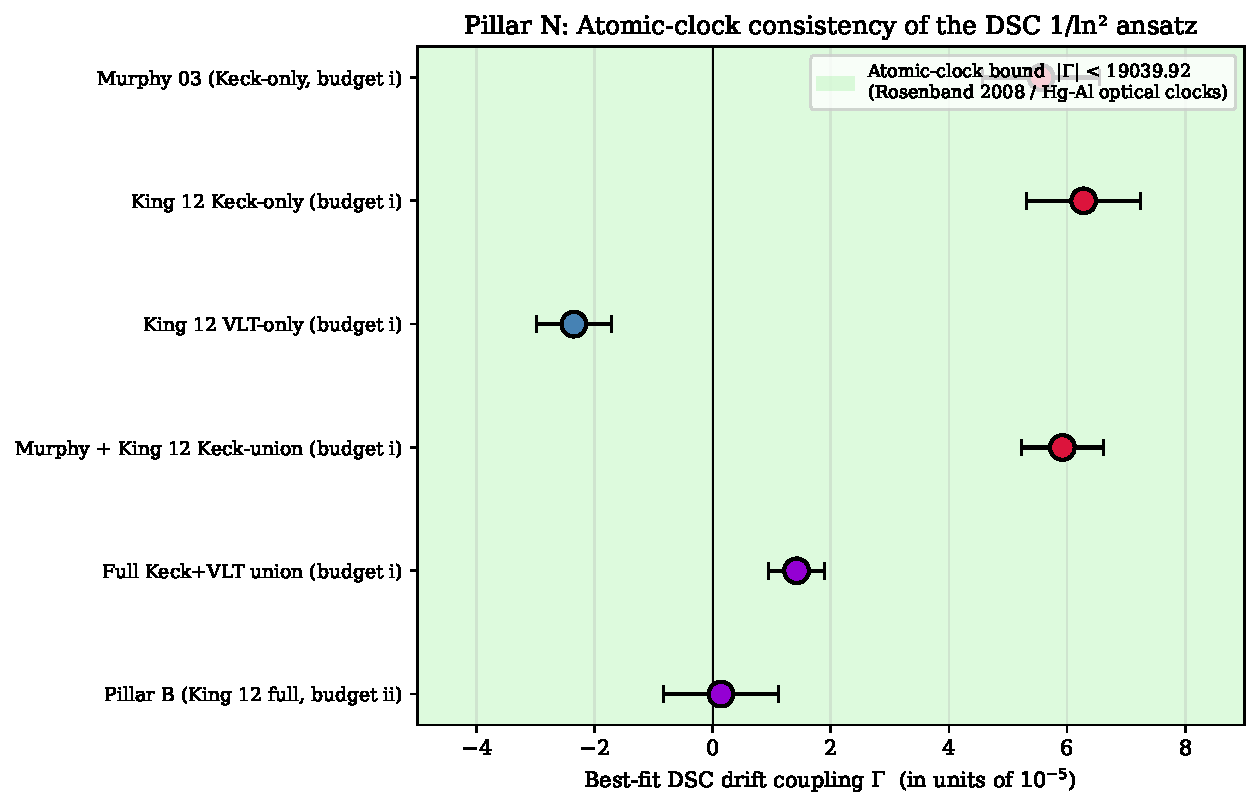
\includegraphics[width=\columnwidth]{fig30_pillar_N_atomic_clock.pdf}
  \caption{Conditional laboratory translation of \cref{eq:alphadot}.
  The horizontal bound $|\Gamma|\lesssim 1.9\times 10^{4}$ follows from the Rosenband et al.\ limit and the derivative of $\xi(t)$.
  The quasar points are the unreconciled submitted values and are not a detection.}
  \label{fig:pillar_N}
\end{figure}

\subsection{Pillar O: previously quoted forecast}
\label{sec:pillarO}

\Cref{tab:forecast} copies the submitted forecast table.
The calculation behind it is the independent-error mock described in \cref{sec:late-method}.
The square-root conversion from a median $\Delta\chi^2$ to a Gaussian-equivalent significance assumes that the likelihood ratio behaves as $\chi^2$ with the degrees of freedom of that mock.
The mock errors are diagonal and proportional to $H$, with no systematic floor.
Under those assumptions the submitted table quotes large separations once the redshift lever arm extends to $z_{\max}\ge 5$.
Those entries are a record of the mock.
They are not a prediction of the significance of a forthcoming survey.
\Cref{fig:pillar_O} shows the same calculation.
The curve separation at $z>2$ is a property of comparing \cref{eq:hubble} with a flat $\Lambda$CDM $H(z)$ that grows roughly as $(1+z)^{3/2}$ in the matter era.
Whether a real catalog can resolve that separation depends on the covariance that this mock omits.

\begin{table}[htbp]
\centering
\caption{Forecast mock as quoted in the submitted manuscript.
Each entry is a median $\sqrt{\Delta\chi^2}$ over 30 draws with independent fractional errors and seed 42.
Scenario~A draws from \cref{eq:hubble}; Scenario~B draws from flat $\Lambda$CDM.
These are not claimed survey significances.}
\label{tab:forecast}
\small
\begin{tabular}{ccc|cc}
\hline
$N$ & $z_{\max}$ & $\sigma_H/H$ & A & B \\
\hline
5  & 3  & 10\% & $2.7$  & $2.9$ \\
5  & 5  & 10\% & $11.4$ & $7.9$ \\
5  & 10 & 10\% & $46.4$ & $12.8$ \\
10 & 5  & 5\%  & $30.3$ & $19.8$ \\
10 & 10 & 5\%  & $123.4$ & $34.7$ \\
20 & 10 & 2\%  & $425.6$ & $118.5$ \\
\hline
\end{tabular}
\end{table}

\begin{figure*}[htbp]
  \centering
  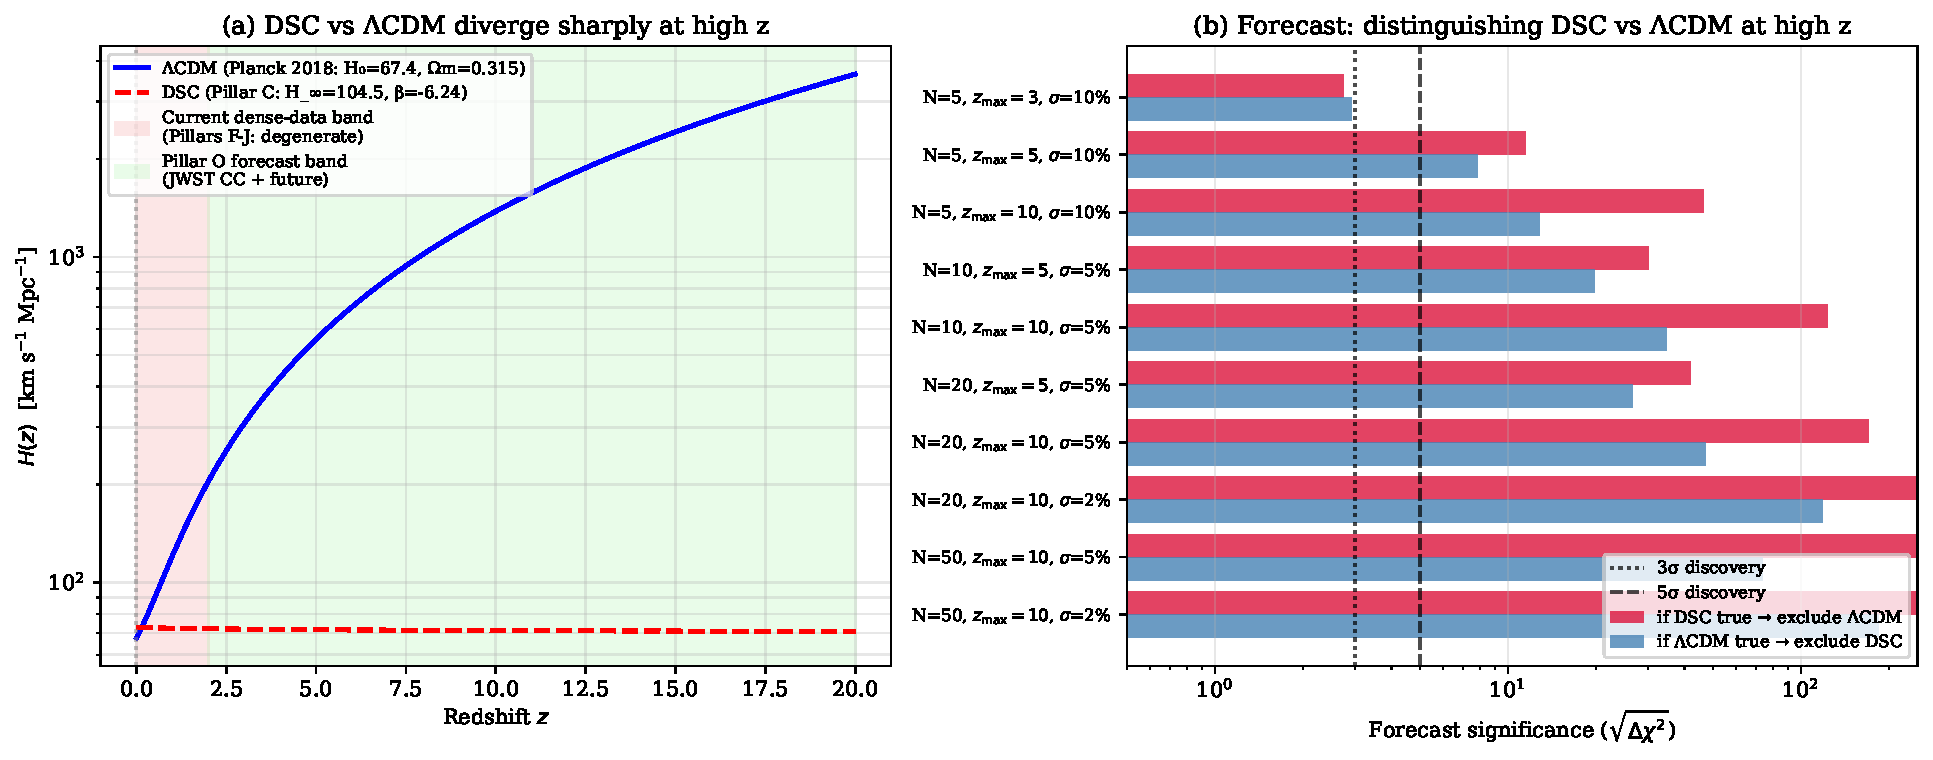
\includegraphics[width=\textwidth]{fig31_pillar_O_forecast.pdf}
  \caption{Previously quoted comparison of \cref{eq:hubble} with flat $\Lambda$CDM.
  Panel~(a) shows the two functions of redshift under the forecast notebook's $\Lambda$CDM clock.
  Panel~(b) shows the independent-error mock of \cref{tab:forecast}.
  The mock has no survey covariance.}
  \label{fig:pillar_O}
\end{figure*}
